\newpage
\section{Расписание. Ведение предварительной записи}

\ifthenelse{\isnamedefined{fullversion} \OR \isnamedefined{regversion}}
{
\subsection{Создание расписания работы врачей} \label{pol_ttbl_new}

Если в ЛПУ организован прием пациентов по предварительной записи или по талонам, необходимо регулярно создавать расписание работы врачей, ведущих амбулаторный прием, и диагностических кабинетов, где ведется прием пациентов по записи,  на последующий период работы ЛПУ. В зависимости от организации работы в конкретном медицинском учреждении, период, на который составляется расписание может быть различным. Рекомендуется создавать расписание на календарный месяц. Однако, возможно создание расписания и на более короткий или более продолжительный период.

Для доступа к созданию и редактированию расписания необходимо нажать на пиктограмму \dm{Формирование графиков} на панели навигации, расположенной по левому краю страницы либо щелкнуть по  плитке \dm{Формирование графиков} на главной странице системы. Будет осуществлен переход на страницу \dm{График врача} (Рисунок \ref{img_pol_ttbl1}).
}{}

\begin{figure}[ht]\centering
 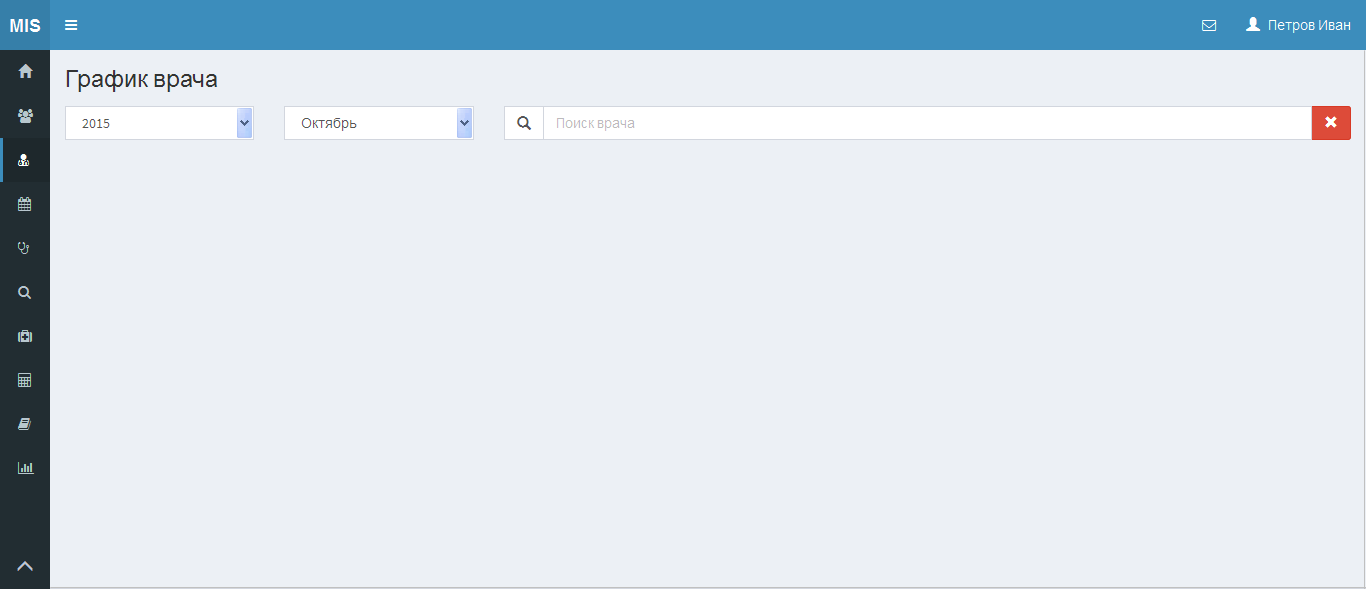
\includegraphics[width = 1\textwidth ,keepaspectratio]{pol_ttbl1}
 \caption{Страница выбора графика работы}
 \label{img_pol_ttbl1}
\end{figure}

\ifthenelse{\isnamedefined{fullversion} \OR \isnamedefined{regversion}}
{
На открывшейся странице необходимо выполнить следующие действия:
\begin{enumerate}
 \item В первом поле выбрать номер года для составления расписания. По умолчанию указывается текущий год.
 \item Во втором поле выбрать месяц, на который планируется составить расписание. По умолчанию указывается текущий месяц.
 \item В третьем поле выбрать сотрудника, для которого планируется составление расписания, либо название диагностического кабинета. По мере ввода текста в данное поле, осуществляется фильтрация списка сотрудников$\slash$кабинетов  по введенному тексту. Отбираются сотрудники, фамилия или специальность которых начинается с введенного буквосочетания, и кабинеты, название которых начинается с указанного буквосочетания. Фамилии сотрудников и названия кабинетов, расписание для которых на выбранный период отсутствует, отображаются в списке зачеркнутыми серым цветом. Следует выбрать запись искомого сотрудника$\slash$кабинета из выпадающего списка, щелкнув по ней левой кнопкой мыши. На экране появится расписание выбранного сотрудника$\slash$кабинета на указанный месяц (Рисунок \ref{img_pol_ttbl2}).   
 \item Нажать кнопку \btn{Редактировать} в левой верхней части страницы. 
\end{enumerate}

\begin{figure}[ht]\centering
 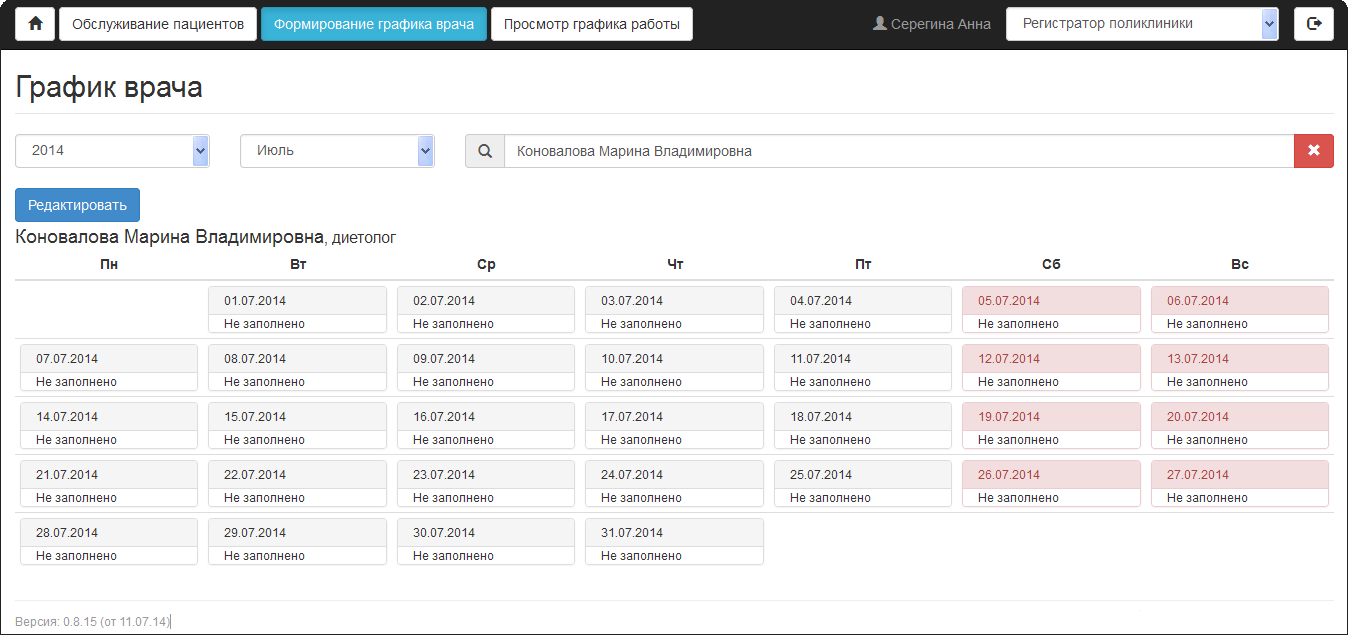
\includegraphics[width = 1\textwidth ,keepaspectratio]{pol_ttbl2}
 \caption{График работы сотрудника}
 \label{img_pol_ttbl2}
\end{figure}

\begin{prim}
 Кнопка 
\includegraphics[scale=0.7]{xdel}, расположенная в правой части поля поиска сотрудника, очищает это поле и снимает фильтрацию со списка сотрудников$\slash$кабинетов соответственно.
\end{prim}
 
В результате выполнения вышеперечисленных действий расписание станет доступно для редактирования, на экране появятся дополнительные кнопки управления расписанием (Рисунок \ref{img_pol_ttbl3}):

\begin{figure}[ht]\centering
 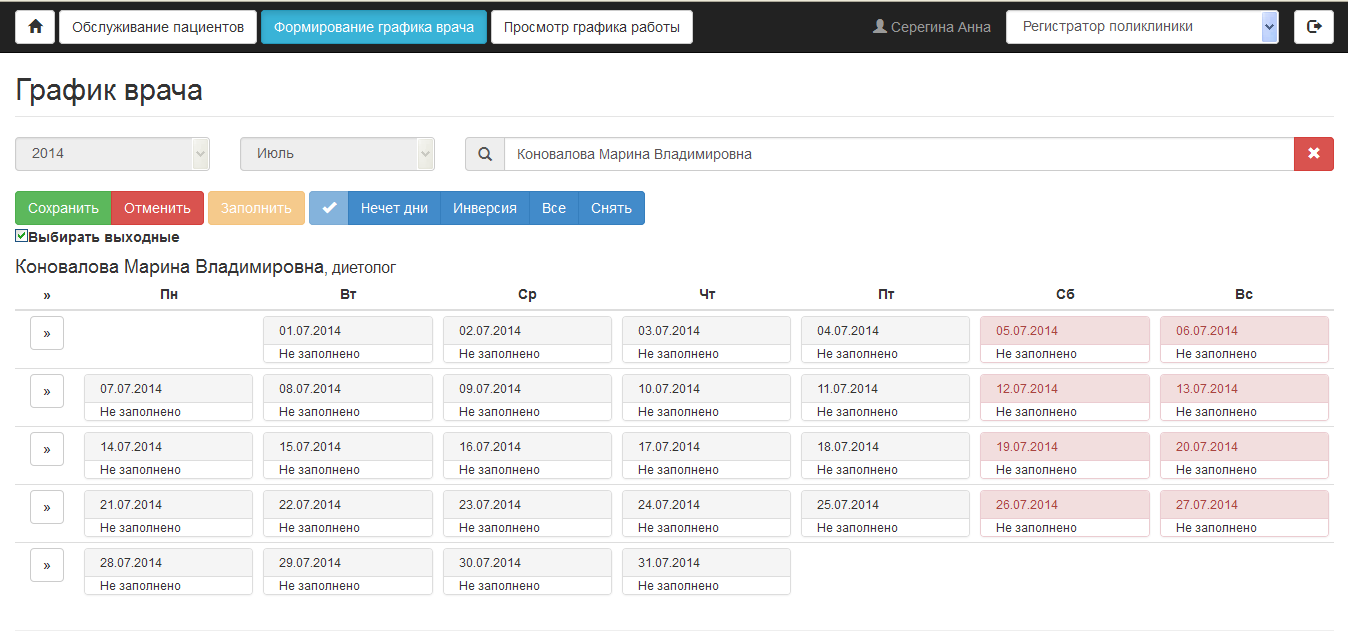
\includegraphics[width = 1\textwidth ,keepaspectratio]{pol_ttbl3}
 \caption{Редактирование расписания сотрудника}
 \label{img_pol_ttbl3}
\end{figure}

По назначению кнопок управления расписанием можно выделить следующие группы:
\begin{enumerate}
 \item Кнопки управления сохранением расписания (группа 1, рисунок \ref{img_pol_ttbl3}). 
 \begin{itemize}
  \item Кнопка \btn{Сохранить} позволяет сохранить созданное расписание сотрудника.
  \item Кнопка \btn{Отменить} осуществляет выход из режима редактирования расписания. Все несохраненные изменения будут потеряны.
 \end{itemize}
 \item Кнопка \btn{Заполнить} открывает окно создания расписание работы сотрудника на выделенные дни. Кнопка доступна, если выделен хотя бы один день расписания.
 \item Кнопки группового выделения (группа 3, рисунок \ref{img_pol_ttbl3}) позволяют выделять или снимать выделение для группы дней по условию:
 \begin{itemize}
  \item Кнопка \btn{Нечет дни} выделяет все нечетные дни месяца. Если флажок \dm{Выбирать выходные} установлен, то выделяются все нечетные дни, включая выходные. В противном случае - только нечетные рабочие дни.
 \item Кнопка \dm{Инверсия} инвертирует выделение дней расписания, т.е. снимает выделение с ранее выделенных дней месяца и выделяет все дни, которые были не выделены. C помощью данной кнопки можно быстро выделить все четные дни месяца. Для этого следует последовательно нажать кнопки \btn{Нечет дни} и \btn{Инверсия}. Если флажок \dm{Выбирать выходные} НЕ установлен, то выходные дни не будут выделяться вне зависимости от того, были ли они выделены до нажатия кнопки \btn{Инверсия}.
 \item Кнопка \btn{Все} позволяет выделить все дни месяца. Если флажок \dm{Выбирать выходные} НЕ установлен, то выделяются все рабочие дни месяца.
 \item Кнопка \btn{Снять} снимает все выделения.
 \end{itemize}
 Можно так же выделять дни в произвольном порядке, щелкая по ним левой кнопкой мыши. Для снятия выделения с дня следует щелкнуть по нему левой кнопкой мыши повторно.
 \item Установленный флажок \dm{Выбирать выходные} позволяет включать в группу выбора выходные дни и составлять на них расписание.
 \item Кнопки 
\includegraphics[scale=0.55]{arr1} (группа 5, рисунок \ref{img_pol_ttbl3}),   позволяют выделить все дни недели, напротив которой расположена кнопка. Если флажок \dm{Выбирать выходные} установлен, то выделяются все дни, в противном случае - только рабочие дни.
 \item Кнопка \btn{Копировать из предыдущего} позволяет скопировать расписание с предыдущего месяца на текущий. При нажатии кнопки со стрелкой вниз справа от данной кнопки, можно выбрать месяц-источник расписания для копирования из нескольких последних месяцев. В случае, если расписание на текущий выбранный период уже заполнено, перед совершением копирования появится диалоговое окно с предупреждением. 
\end{enumerate}

При заполнении расписания последовательность действий следующая: 
\begin{enumerate}
 \item \label{n2} Необходимо выделить один или несколько дней, расписание на которые совпадает, с помощью кнопок, перечисленных выше, либо щелчком левой кнопки мыши и нажать кнопку \btn{Заполнить} на странице \dm{График врача}. Появится всплывающее окно \dm{Заполнение расписания} (Рисунок \ref{img_pol_ttbl4}). В верхней части открывшегося окна будут перечислены дни, на которые будет сформировано расписание в результате текущей операции. 

 \begin{figure}[ht]\centering
  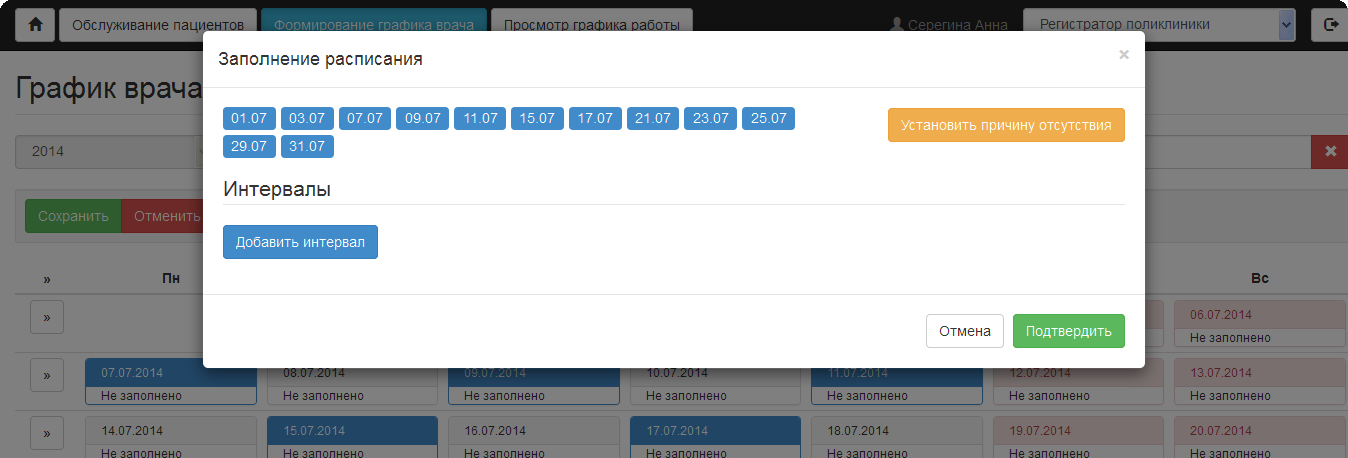
\includegraphics[width = 1\textwidth ,keepaspectratio]{pol_ttbl4}
  \caption{Окно <<Заполнение расписания>>}
  \label{img_pol_ttbl4}
 \end{figure}

 \item \label{n1} Следует нажать кнопку \btn{Добавить интервал} и заполнить появившиеся поля (Рисунок \ref{img_pol_ttbl5}):
 \begin{itemize}
  \item \dm{Тип} -- тип приема выбирается из списка (<<Амбулаторно>> или <<Hа дому>>);
  \item \dm{Начало приема} -- время начала работы врача по обслуживанию обращений выбранного типа;
  \item \dm{Окончание приема} -- время окончания работы врача по обслуживанию обращений выбранного типа;
  \item \dm{План приема} -- плановое количество пациентов, которых должен принять врач$\slash$кабинет за указанный интервал. Соответствует количеству талонов, которые будут созданы на текущий день для выбранного типа приема. 
  \item \dm{Сверх плана} -- допустимое количество пациентов, которые могут быть записаны дополнительно, сверх планового числа талонов;
  \item \dm{Вне очереди} -- допустимое количество экстренных пациентов, которые могут быть приняты без талона в течении заданного интервала.
  \item \dm{Кабинет} -- кабинет, в котором ведется прием. Поле доступно только, если выбран амбулаторный тип приема. Кабинет может быть выбран из раскрывающегося списка кабинетов ЛПУ. Вверху раскрывающегося списка предусмотрено поле поиска кабинета в списке.
  \item \dm{Источник финансирования} -- источник финансирования, по которому осуществляется прием. Если источник финансирования выбран, то в данный интервал осуществляется прием пациентов только по указанному источнику финасирования. Если значение не выбрано, то возможен прием всех пациентов.
 \end{itemize}
 Поля \dm{Тип}, \dm{Начало приема}, \dm{Окончание приема}, \dm{План приема} являются обязательными для заполнения.  Для амбулаторного типа приема обязательным так же является поле \dm{Кабинет}.

\begin{figure}[ht]\centering
 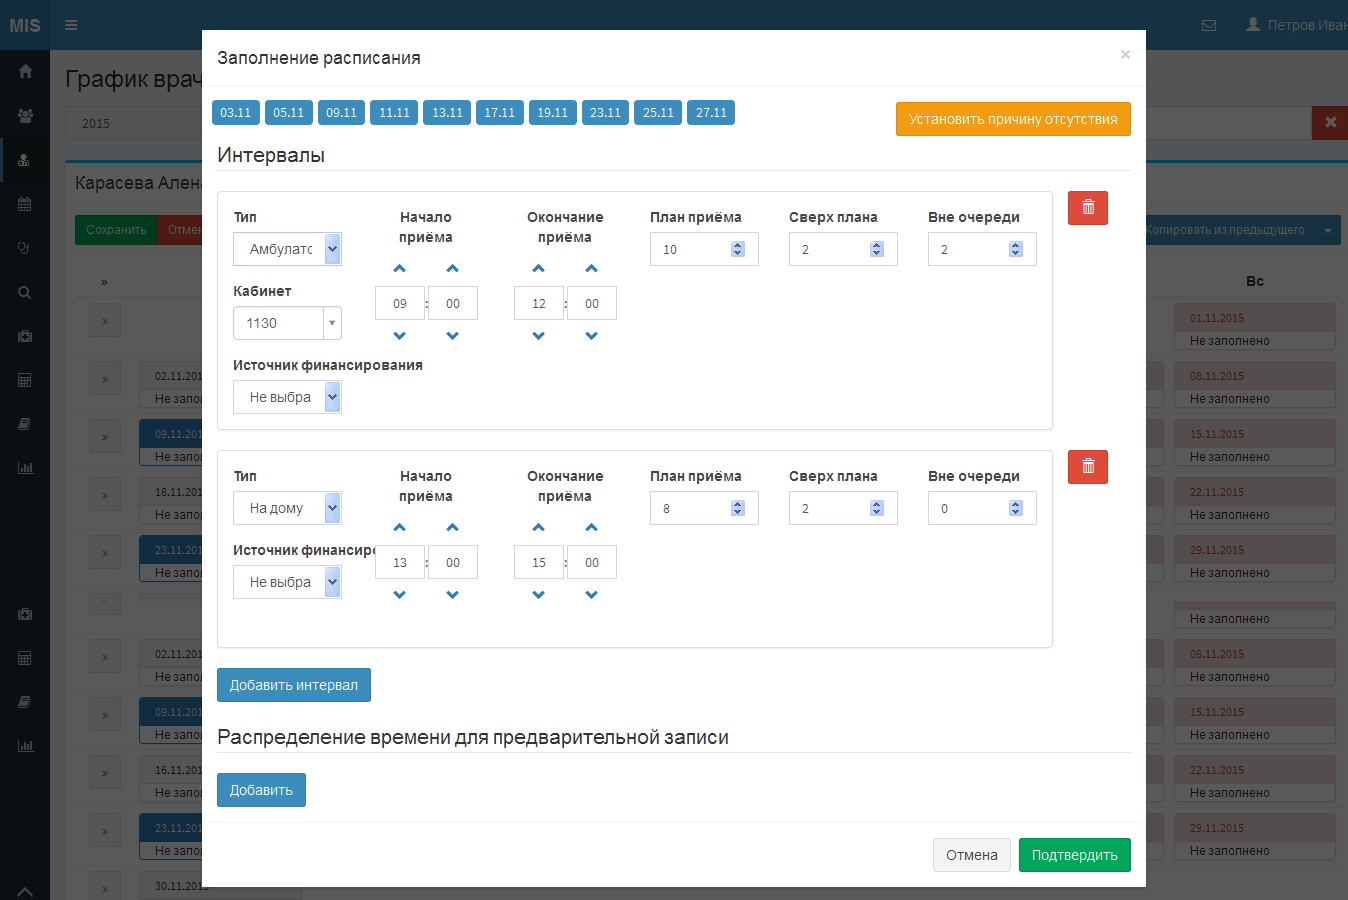
\includegraphics[width = 1\textwidth ,keepaspectratio]{pol_ttbl5}
 \caption{Окно <<Заполнение расписания>> после внесения данных}
 \label{img_pol_ttbl5}
\end{figure}

 \item Повторить п. \ref{n1} для добавления нужного числа интервалов приема. Допускается добавление нескольких интервалов в рамках одного дня приема, в том числе нескольких интервалов одного типа (например, можно добавить 2 интервала одного типа, если прием ведется с перерывом). 
 
 \item При необходимости квотирования времени приема для записи можно нажать кнопку \btn{Добавить} в разделе \dm{Распределение времени для предварительной записи} и разделить время приема выбранного дня между различными типами записи. Допускается назначение нескольких типов записи на один и тот же интервал. Для добавления нескольких записей квотирования следует повторно нажимать кнопку \btn{Добавить} внизу окна и заполнять появившиеся поля до достижения необходимого количества записей:
 \begin{itemize}
 	\item \dm{Тип} -- тип записи, выбирается из раскрывающегося списка. Поле обязательно для заполнения. Возможны следующие типы записей: 
 	\begin{itemize}
 		\item Запись из регистратуры -- указанный интервал доступен для записи регистраторами поликлиники;
 		\item Запись врачем на повторный прием -- на указанный интервал врач может записать пациента к себе на повторный прием;
 		\item Межкабинетная запись -- на указанный интервал другие врачи могут записывать своих пациентов к данному врачу;
 		\item Запись из других ЛПУ -- на указанный интервал могут быть записаны пациенты из внешних ЛПУ;
 		\item Запись через Портал -- на указанный интервал пациенты могут записаться самостоятельно через Интернет.		
 	\end{itemize}
 	\item \dm{Начало периода} -- время начала интервала записи;
 	\item \dm{Окончание периода} -- время окончания интервала записи;	
 \end{itemize}
 Для удаления одного из интервалов, необходимо нажать кнопку 
\includegraphics[scale=0.7]{delb} напротив соответствующей строки. 
 
 \item \label{n3} После заполнения расписания окно будет выглядеть следующим образом (Рисунок \ref{img_pol_ttbl5}). Следует нажать кнопку \btn{Подтвердить} в правом нижнем углу окна, после чего оно будет закрыто, а в окне \dm{График врача} расписание на выбранные дни будет заполнено в соответствии с заданным шаблоном. 
 \item При необходимости повторить шаги \ref{n2} -- \ref{n3} нужное число раз для заполнения расписания на весь требуемый период. По окончании заполнения, страница формирования графика врача примет следующий вид (Рисунок \ref{img_pol_ttbl6}). 
 \item Следует нажать кнопку \btn{Сохранить} для внесения расписания в БД. 
\end{enumerate}

\begin{figure}[ht]\centering
 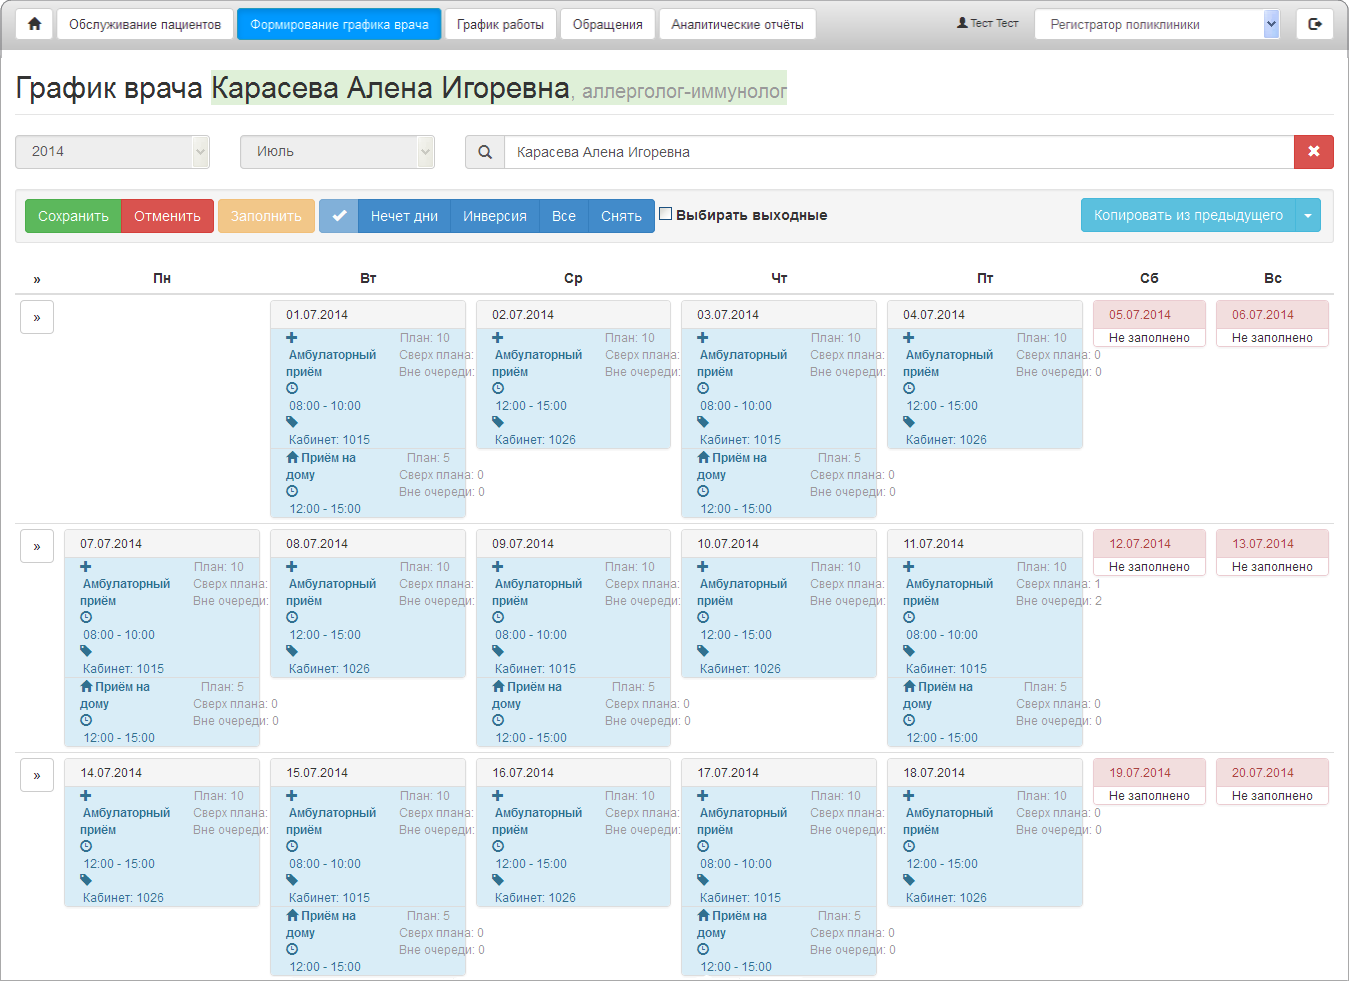
\includegraphics[width = 1\textwidth ,keepaspectratio]{pol_ttbl6}
 \caption{Заполненное расписание сотрудника}
 \label{img_pol_ttbl6}
\end{figure}

\subsubsection{Регистрация отсутствий сотрудников}

Если врач не может вести прием по какой-либо причине, необходимо отметить его отсутствие в расписании. Для этого следует открыть расписание сотрудника на соответствующий период на редактирование, выбрать дни отсутствия и нажать кнопку \btn{Заполнить}. Откроется всплывающее окно \dm{Заполнение расписания}. В правом верхнем углу окна нужно нажать кнопку \btn{Установить причину отсутствия} и в появившемся под кнопкой поле выбрать из раскрывающегося списка причину отсутствия. Далее следует нажать кнопку \btn{Подтвердить} в правом нижнем углу окна. Расписание сотрудника на выбранные дни будет удалено, а в полях дней отсутствия будет указана выбранная причина (Рисунок \ref{img_pol_ttbl7}). После сохранения  расписание сотрудника станет недоступным для записи на дни отсутствия.

\begin{vnim}
 Не забудьте сохранить расписание после внесения информации об отсутствиях кнопкой \btn{Сохранить}.
\end{vnim} 

\begin{figure}[ht]\centering
 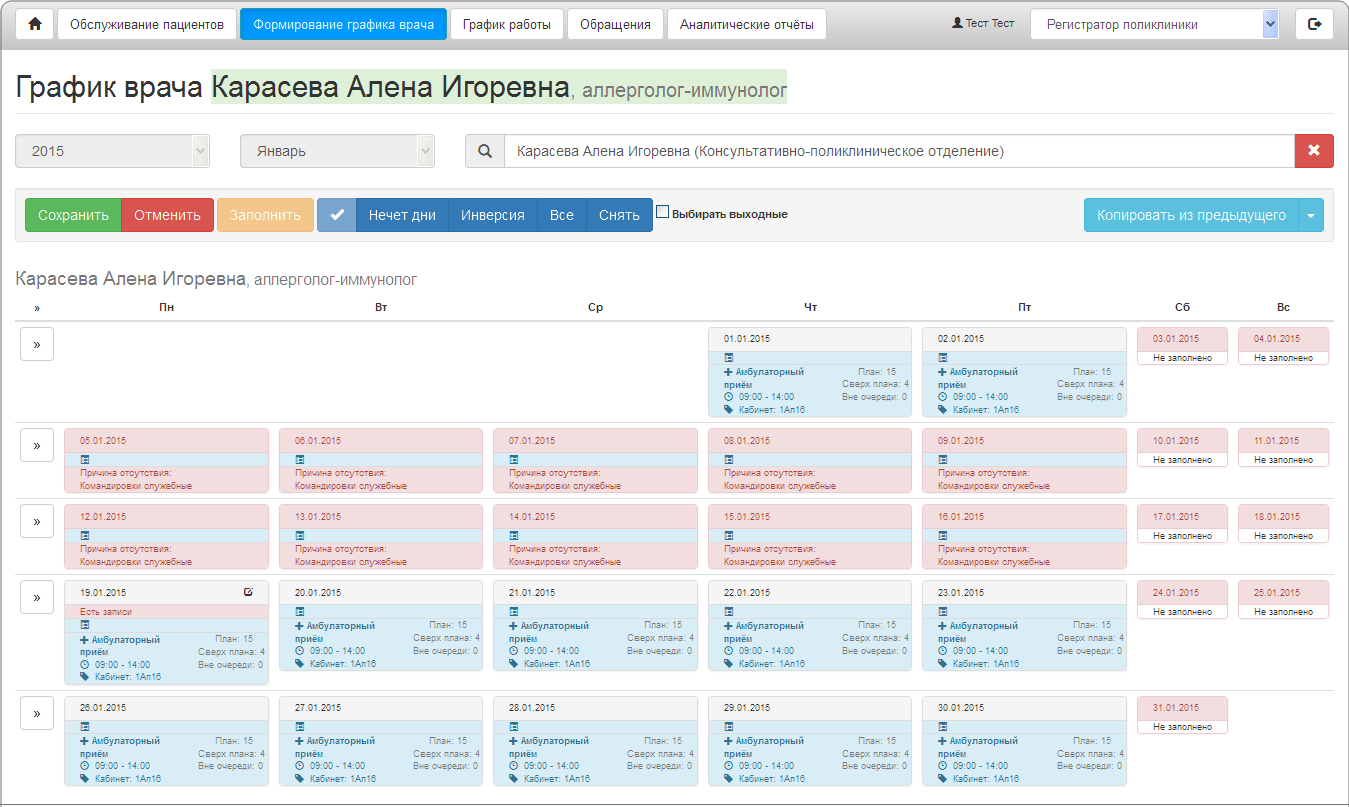
\includegraphics[width = 1\textwidth ,keepaspectratio]{pol_ttbl7}
 \caption{Отсутствия сотрудника}
 \label{img_pol_ttbl7}
\end{figure}

Если необходимо отменить запись об отсутствии сотрудника, следует выделить дни, в которые нужно отменить ранее установленное отсутствие и нажать кнопку \btn{Заполнить}. Появится всплывающее окно \dm{Заполнение расписания}. В правом верхнем углу появившегося окна следует нажать кнопку \btn{Убрать причину отсутствия} и нажать кнопку \btn{Подтвердить}. Запись об отсутствии сотрудника будет удалена, однако расписание сотрудника на эти дни нужно будет создать заново.

Если на определенный день в расписании сотрудника записан хотя бы один пациент, то данный день недоступен для выбора при редактировании расписания. В правом верхнем углу таких дней установлен значок 
\includegraphics[scale=1]{ttblne}. Если необходимо установить отсутствие на такой день, то следует щелкнуть левой кнопкой мыши по значку 
\includegraphics[scale=1]{ttblne} и в появившемся всплывающем окне <<Блокировка дня и перенос пациентов>> выбрать причину отсутствия из раскрывающегося списка, после чего нажать кнопку \btn{Подтвердить}. Откроется окно, где необходимо выполнить перенос записей всех пациентов на другие дни (Рисунок \ref{img_pol_ttbl_remove}). 

\begin{figure}[ht]\centering
 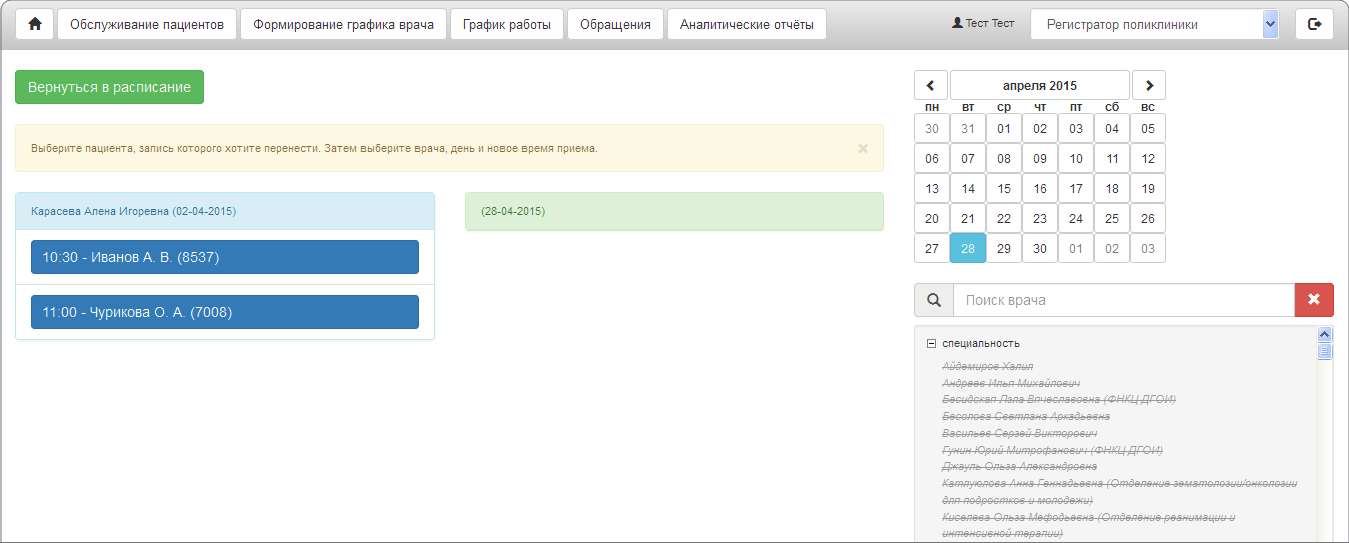
\includegraphics[width = 1\textwidth ,keepaspectratio]{pol_ttbl_remove}
 \caption{Перенос пациенттов}
 \label{img_pol_ttbl_remove}
\end{figure}

Порядок действий по переносу пациентов должен быть следующий: 

\begin{enumerate}
 \item Выбрать пациента из списка в левой части страницы.
 \item Найти расписание врача в списке в правой части страницы, воспользовавшись поиском или вручную. Перенос возможен как к текущему, так и к другому врачу.
 \item В календаре, расположенном в правом верхнем углу страницы, выбрать дату, на которую будет осуществляться перенос. В расписании на выбранный день должны быть свободные интервалы для записи.
 \item В открывшемся расписании в центральной части страницы указать свободный интервал, на который следует перенести пациента, выбранного на шаге 1. Пациент будет перенесен.
 \item Повторить шаги 1 -- 4 для остальных пациентов из списка в левой части страницы.
\end{enumerate}

}{}

\subsection{Просмотр расписания} \label{pol_ttbl_view}

Просмотреть расписание работы сотрудников$\slash$кабинетов можно, щелкнув левой кнопкой мыши по пиктограмме \dm{График работы} на панели навигации либо нажав на плитку \dm{Просмотр графиков} на главной странице системы. Будет осуществлен переход на страницу \dm{График работы} (Рисунок \ref{img_pol_ttbl1}).

\begin{prim}
 Просмотр расписания доступен так же при записи пациента на прием.
\end{prim}

В верхней части страницы необходимо выбрать год и месяц, на которые нужно посмотреть расписание, а так же фамилию сотрудника, расписание которого требуется просмотреть либо название кабинета  \ifthenelse{\isnamedefined{fullversion} \OR \isnamedefined{regversion}}{(см. раздел \ref{pol_ttbl_new})}{. Фамилии сотрудников и названия кабинето,для которых отсутствует расписание на выбранный период, отображаются в списке зачеркнутыми серым цветом .} После этого ниже, на текущей  странице отобразится расписание выбранного сотрудника$\slash$кабинета (Рисунок \ref{img_pol_ttblview}). По умолчанию будет открыто расписание на текущую неделю выбранного месяца. 

\begin{figure}[ht]\centering
 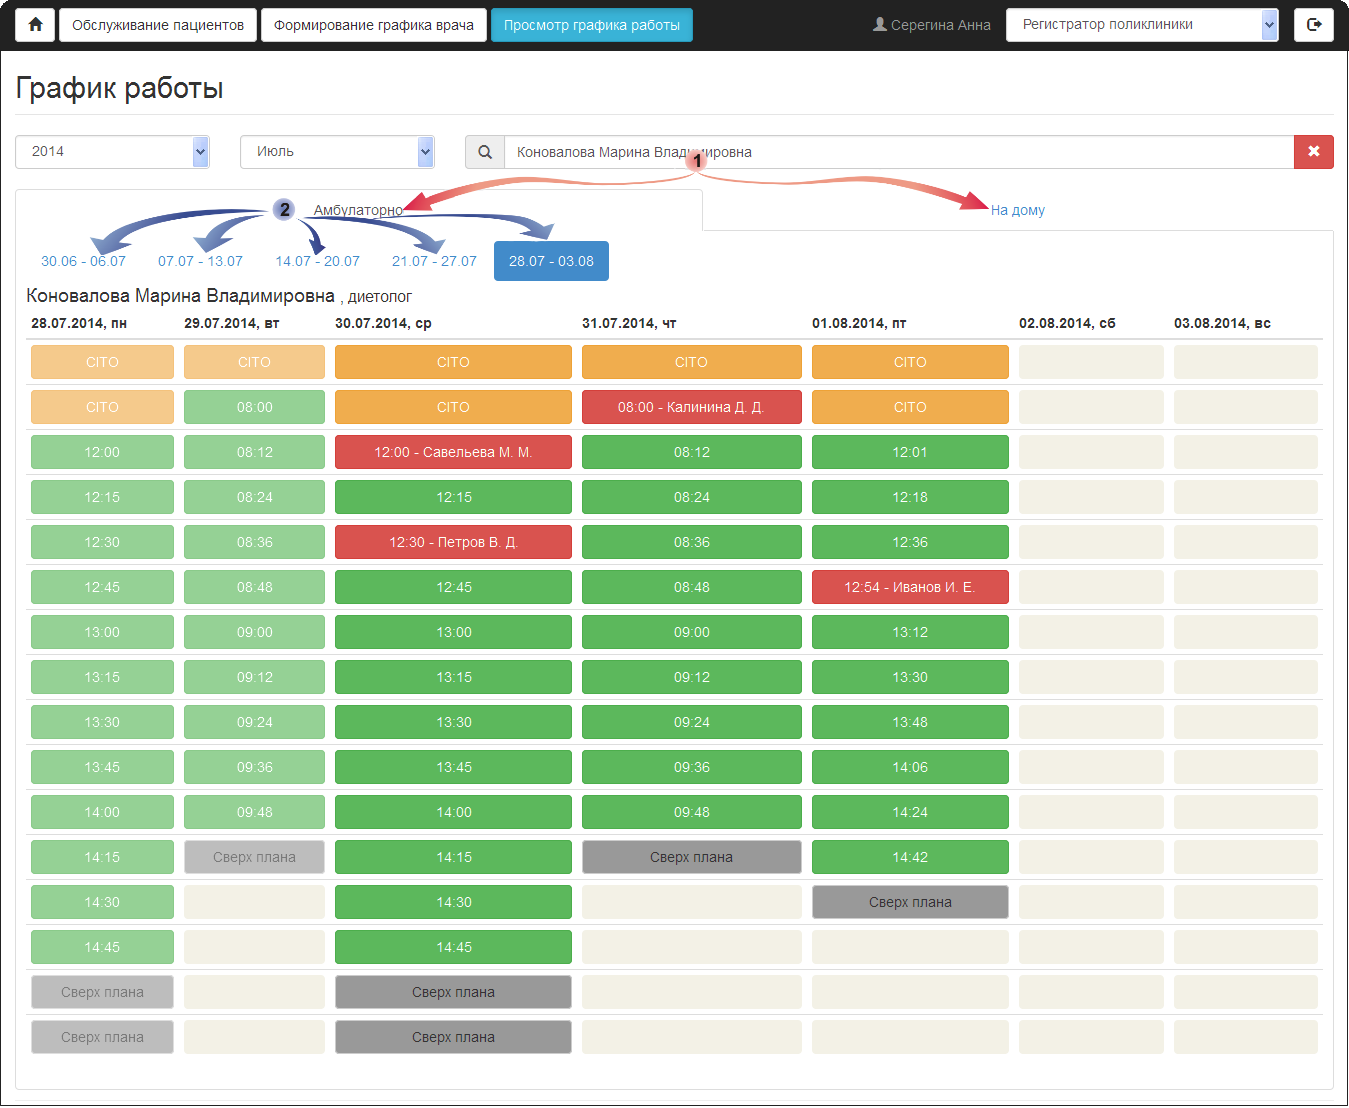
\includegraphics[width = 1\textwidth ,keepaspectratio]{pol_ttblview}
 \caption{Просмотр расписания}
 \label{img_pol_ttblview}
\end{figure}

Для просмотра расписания амбулаторного приема должна быть активирована вкладка \dm{Амбулаторно}. Для просмотра графика обслуживания квартирных вызовов следует осуществить переход на вкладку \dm{На дому} (Рисунок \ref{img_pol_ttblview}, [1]). Ниже, под названием вкладки, отображается список недель выбранного месяца (Рисунок \ref{img_pol_ttblview}, [2]). Для просмотра расписания на другую неделю, следует выбрать ее, щелкнув по ней левой кнопкой мыши.

В основной части страницы отображается список интервалов приема выбранного врача$\slash$кабинета на выбранную неделю. В зависимости от доступности и назначения интервалы имеют следующие цвета и обозначения. Если для интервала задан определенный источник финансирования, то он будет окрашен в цвет, соответствующий этому источнику (Рисунок \ref{img_pol_ttblview}, [3]). Если источник финансирования для интервала не задан, то он имеет следующую раскраску:

\begin{itemize}
 \item \dm{Зеленый цвет} -- свободные интервалы приема, на которые могут быть записаны пациенты. На каждом интервале указано время начала приема;
 \item \dm{Оранжевый цвет} с надписью <<CITO>> обозначает интервалы, предназначены для записи экстренных пациентов;
 \item \dm{Серый цвет} с надписью <<Сверх плана>> -- на данный интервал допустимо записать пациента сверх плановой нормы приема;
 \item \dm{Синий цвет} обозначает интервалы, на которые уже записаны пациенты. На каждом интервале указывается время начала приема и фамилия записанного пациента. Щелкнув по кнопке 
\includegraphics[scale=0.7]{pers}, расположенной в правой части каждого занятого интервала, можно перейти к регистрационной карте записанного пациента;
\end{itemize}

Интервалы прошедших периодов, на которые уже невозможна запись, имеют ту же раскраску, что и активные интервалы, но более бледного тона.

Из данного раздела можно осуществлять запись пациентов на прием. Для этого нужно щелкнуть левой кнопкой мыши по интервалу, доступному для записи, в появившемся всплывающем окне ввести данные пациента (фамилию, дату рождения, номер документа и т.п.) в поле поиска и нажать кнопку \btn{Найти} или клавишу \keys{Enter} на клавиатуре (Рисунок \ref{img_pol_zapnew}). В нижней части всплывающего окна появится список пациентов, найденных согласно условиям поиска (Рисунок \ref{img_pol_zapclt}). Необходимо выбрать из списка одного из пациентов и нажать кнопку \btn{Далее}.   

\begin{figure}[ht]\centering
 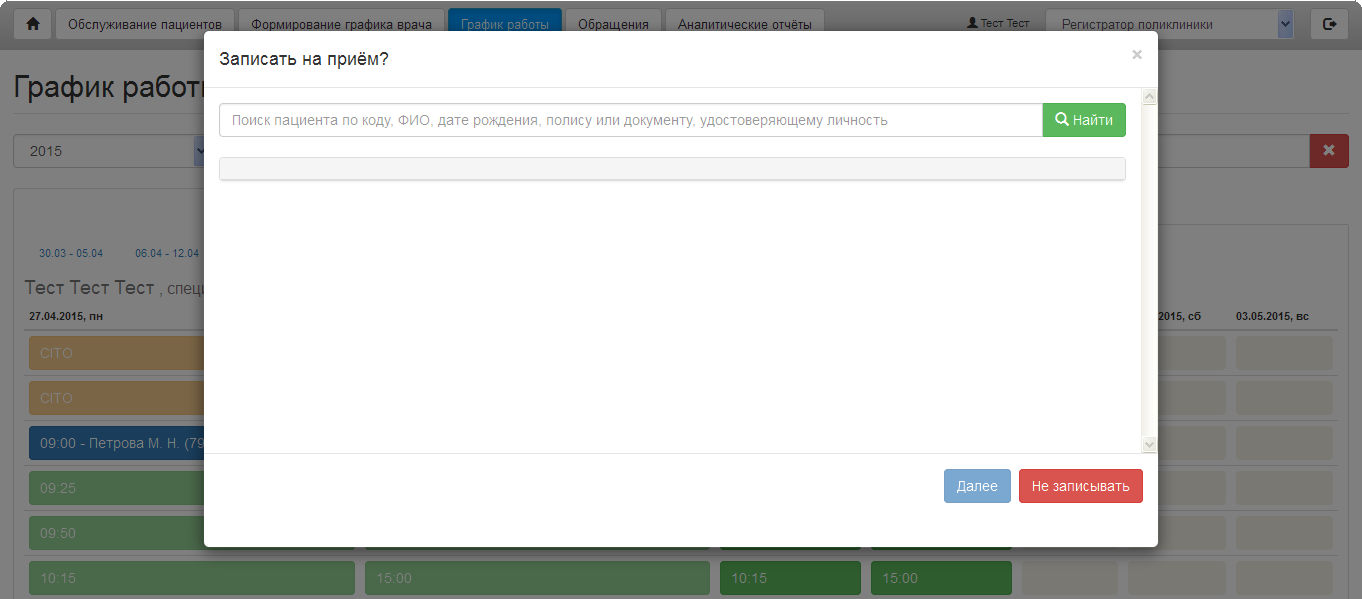
\includegraphics[width = 1\textwidth ,keepaspectratio]{pol_zapnew}
 \caption{Всплывающее окно записи пациента на прием в разделе <<График работы>>}
 \label{img_pol_zapnew}
\end{figure}

На следующем шаге требуется выбрать тип обращения из раскрывающегося списка и снова нажать кнопку \btn{Далее}. Пациент будет записан на выбранный интервал. 

На любом из шагов можно отказаться от записи пациента, нажав кнопку \btn{Не записывать} во всплывающем окне. 

\begin{figure}[ht]\centering
 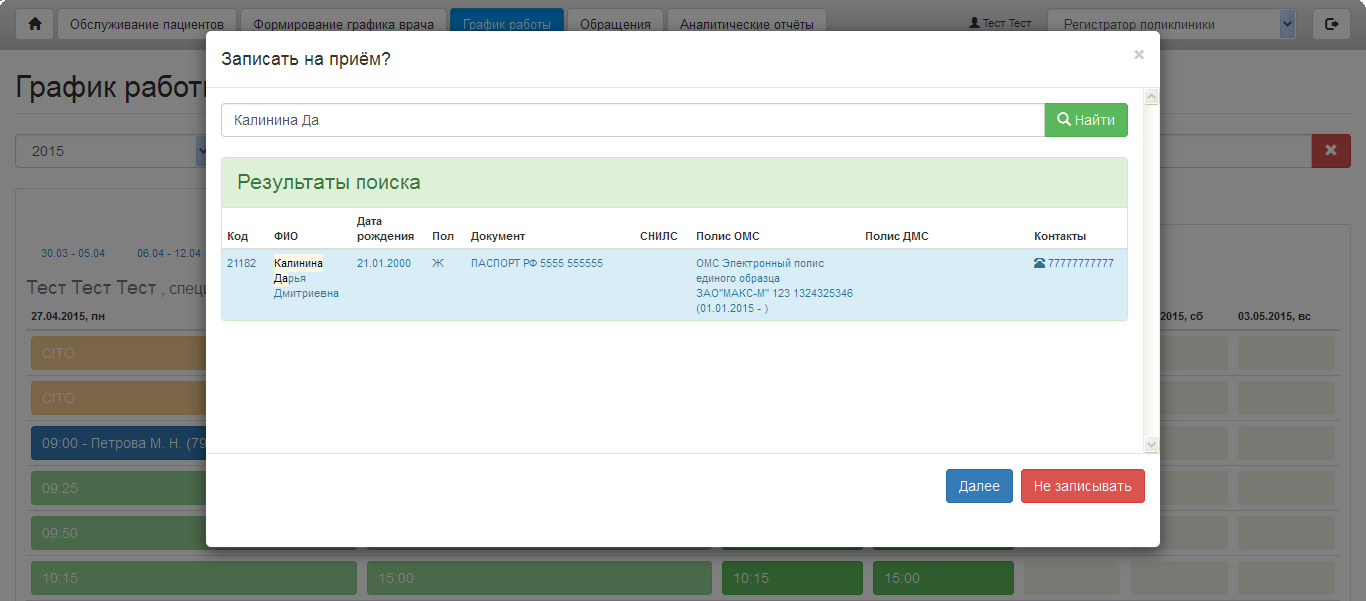
\includegraphics[width = 1\textwidth ,keepaspectratio]{pol_zapclt}
 \caption{Выбор пациента для записи на прием в разделе <<График работы>>}
 \label{img_pol_zapclt}
\end{figure}

Для отмены ранее зарегистрированной записи можно щелкнуть по соответствующему интервалу (синего цвета) в расписании и в появившемся окне (Рисунок \ref{img_pol_zapcancel}) нажать кнопку \btn{Отменить запись}. Запись пациента будет отменена, а интервал освобожден.

\begin{figure}[ht]\centering
 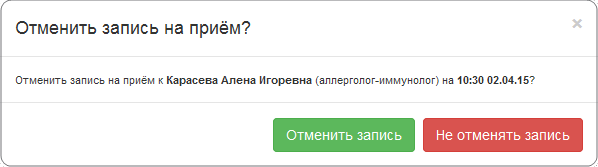
\includegraphics[width = 0.6\textwidth ,keepaspectratio]{pol_zapcancel}
 \caption{Окно отмены записи пациента}
 \label{img_pol_zapcancel}
\end{figure}


\subsection{Предварительная запись на прием}\label{pol_predvz}

\ifthenelse{\isnamedefined{fullversion} \OR \isnamedefined{regversion}}{
Предварительная запись пациентов на прием осуществляется на странице обслуживания пациентов. Для перехода на эту страницу необходимо щелкнуть левой кнопкой мыши по пиктограмме \dm{Обслуживание пациентов} на панели навигации, либо нажать на блок \dm{Обслуживание пациентов} на главной странице системы (Рисунок \ref{img_gen_main}).}
{Предварительная запись пациентов на прием осуществляется из раздела \dm{Прием пациентов} (будет подробно рассмотрено далее) или из раздела \dm{Поиск пациентов}.} 

Последовательность действий при записи пациента на прием \ifthenelse{\isnamedefined{doctorversion}} {из раздела \dm{Поиск пациентов}}{} должна быть следующая:
\begin{enumerate}
 \item \label{n4} Необходимо найти пациента в картотеке (см. раздел \ref{cl_find}) \ifthenelse{\isnamedefined{fullversion} \OR \isnamedefined{regversion}}{Если пациент не был зарегистрирован ранее, его следует зарегистрировать (см. раздел \ref{cl_new}) в  БД.}{}
 \item Если пациент найден в БД, нужно щелкнуть левой кнопкой мыши по записи о нем в списке найденных пациентов и в появившемся всплывающем окне (Рисунок \ref{img_cl_contrwin}) нажать кнопку \btn{Записать на прием} или кнопку 
\includegraphics[scale=0.55]{rec} в правом верхнем углу окна. Для вновь зарегистрированного пациента можно нажать кнопку \btn{Записать на прием} в правом верхнем углу регистрационной карточки пациента. Откроется страница \dm{Запись пациента на прием}.  
 \item В правой верхней части страницы, в поле поиска врача, нужно ввести фамилию или специальность врача либо название диагностического кабинета. По мере ввода данных в поле поиска, список врачей и кабинетов, расположенный ниже, будет фильтроваться согласно условиям поиска.
 
 \begin{prim}
   Кнопка  
\includegraphics[scale=0.7]{xdel} в поле поиска врача позволяет очистить данное поле, в результате чего, отображается полный список сотрудников ЛПУ и диагностических кабинетов. Кнопка  
\includegraphics[scale=0.7]{xdel} напротив фамилии пациента, закрывает страницу предварительной записи для данного пациента.
  \end{prim}
  
 \item \label{n5} Далее следует установить флажок напротив одной или нескольких фамилий врачей, к которым требуется записать пациента. На экране появится расписание выбранного сотрудника (или сотрудников) на текущую неделю (Рисунок \ref{img_pol_zapttbl}). Цветовые обозначения интервалов здесь аналогичны описанным в разделе \ref{pol_ttbl_view} Единственное отличие состоит в том, что при записи на прием  синим цветом обозначены интервалы, на которые записан текущий пациент на выбранной неделе. Если интервал занят другим пациентом, то он вовсе не отображается на данной странице.
 
 \begin{figure}[ht]\centering
  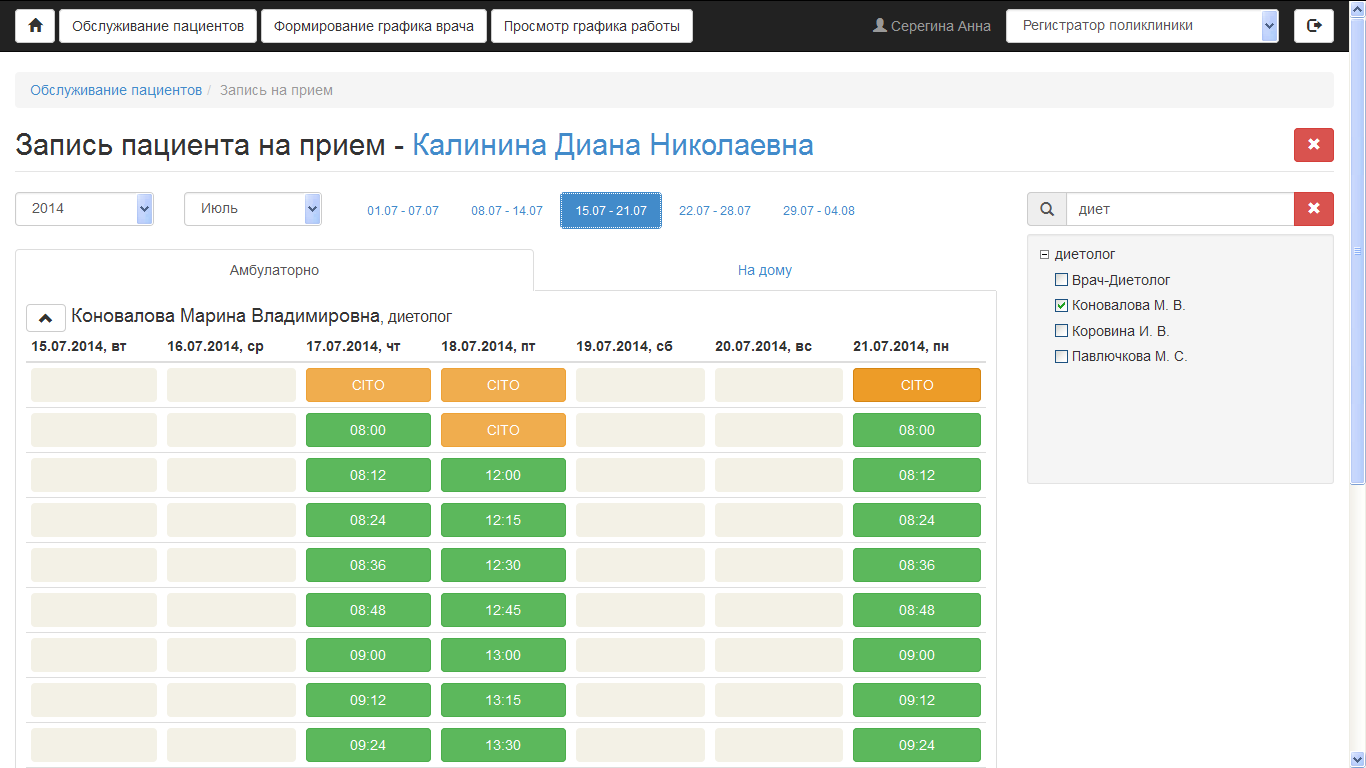
\includegraphics[width = 1\textwidth ,keepaspectratio]{pol_zapttbl}
  \caption{Запись пациента на прием}
  \label{img_pol_zapttbl}
 \end{figure}
 
 \item В случае наличия свободных талонов, нужно щелкнуть по одному из них левой кнопкой мыши. Если свободные для записи интервалы отсутствуют, можно сменить неделю, выбрав соответствующие год, месяц и неделю в верхней части страницы.
 \item После выбора свободного интервала в появившемся всплывающем окне следует выбрать из раскрывающегося списка тип обращения, заполнить поле \dm{Комментарий} (при необходимости) и нажать кнопку \btn{Записать}. Выбранный интервал окрасится в синий цвет.
\end{enumerate}

 \begin{figure}[ht]\centering
  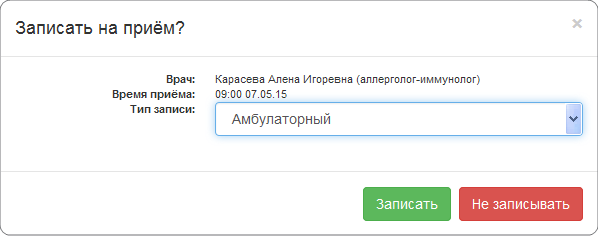
\includegraphics[width = 0.6\textwidth ,keepaspectratio]{pol_tpobr}
  \caption{Запись на прием}
  \label{img_pol_tpobr}
 \end{figure}

Если одновременно было выбрано несколько сотрудников в списке для просмотра расписания, то их расписания будут отображаться последовательными блоками. Для просмотра расписания следующего сотрудника можно воспользоваться полосой прокрутки либо скрыть расписание предыдущего сотрудника, нажав кнопку \includegraphics[scale=0.7]{rollup}, слева от его фамилии.

Если для выбранного пациента ранее были зарегистрированы предварительные записи к другим специалистам на выбранную неделю, то расписания этих врачей, будет всегда отображаться при последующих записях на прием внизу списка в свернутом виде (Рисунок \ref{img_pol_zap2ttbl}) таким образом, что будут видны дата и время предварительных записей только текущего пациента. Развернуть расписание можно, нажав кнопку 
\includegraphics[scale=0.7]{rolldown} слева от фамилии сотрудника.

 \begin{figure}[ht]\centering
  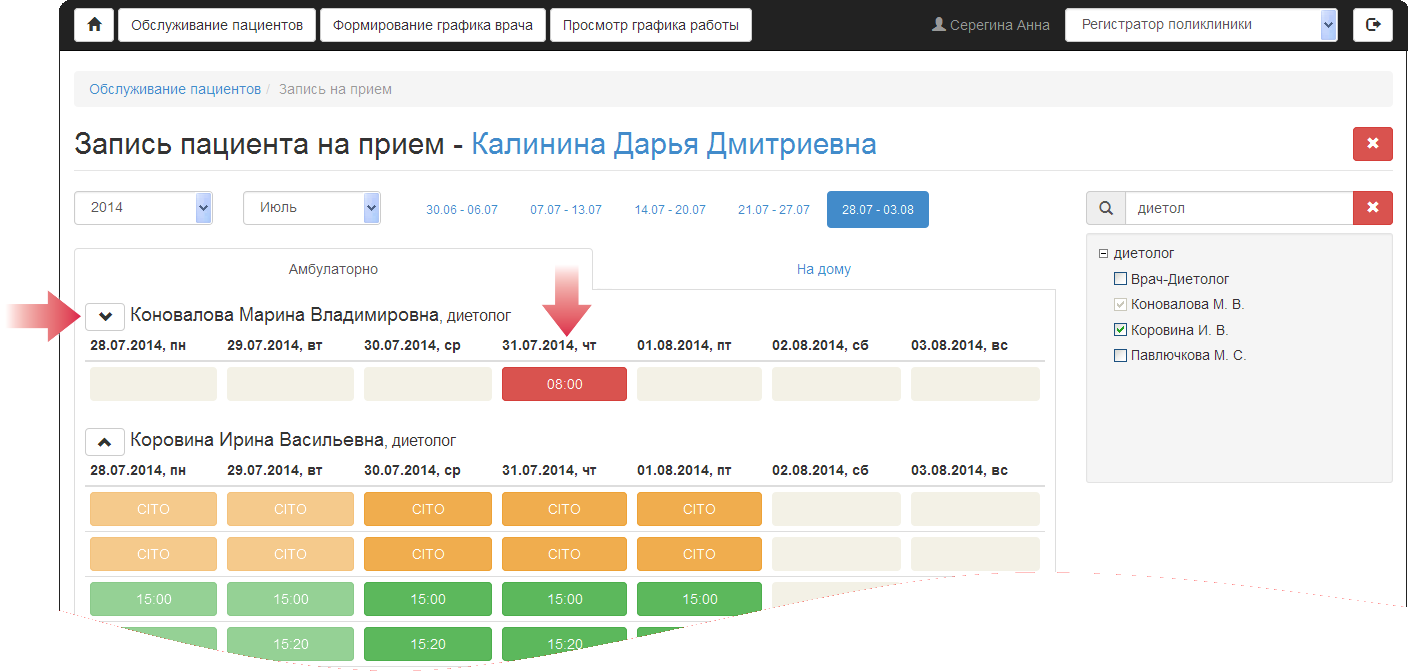
\includegraphics[width = 1\textwidth ,keepaspectratio]{pol_zap2ttbl}
  \caption{Отображение ранее выполненных предварительных записей}
  \label{img_pol_zap2ttbl}
 \end{figure}
     
В \tmisp~реализована возможность экстренной записи и записи сверх нормы на выбранную дату. Для записи экстренного пациента, нужно выбрать в расписании талон оранжевого цвета с надписью <<CITO>>. Талоны <<CITO>> всегда располагаются самыми первыми в расписании врача. Если экстренные талоны отсутствую, то для данного врача не предусмотрен прием экстренных пациентов вне очередности приема.

Для записи пациентов сверх нормы нужно выбрать в расписании талон серого цвета с надписью <<Сверх плана>>. Талоны данного типа всегда распологаются в самом конце списка интервалов выбранного врача на соответствующий день. Если талоны <<Сверх нормы>> отсутствуют, то данный врач$\slash$кабинет не осуществляет прием сверх плана либо все они уже заняты. 

\begin{prim}
Количество экстренных пациентов и пациентов сверх плана, которые могут быть записаны к данному врачу$\slash$кабинет на текущий день, настраивается при создании расписания работы каждого врача$\slash$кабинета индивидуально. 
\end{prim}

Для отмены предварительной записи текущего пациента нужно щелкнуть по соответствующему талону синего цвета на странице записи пациентов на прием (Рисунок \ref{img_pol_zapttbl}) и в появившемся всплывающем окне <<Отменить запись на прием?>> нажать кнопку \btn{Отменить запись}. Запись пациента на прием будет отменена, выбранный интервал осободится и окрасится в соответствующий его состоянию цвет.

\subsection{Вызов врача на дом} \label{pol_home}

Механизм регистрации вызовов врача на дом в \tmisp~полностью аналогичен предварительной записи на прием в поликлинике. Для регистрации вызова на дом необходимо выполнить шаги \ref{n4} -- \ref{n5}, описанные в п. \ref{pol_predvz} Далее следует перейти на вкладку \dm{На дому} (Рисунок \ref{img_pol_ttbl1}, [1]), а затем щелкнуть левой кнопкой мыши по любому свободному интервалу на требуемый день, в открывшемся окне выбрать из раскрывающегося списка тип обращения и нажать кнопку \btn{Далее} в окне подтверждения записи на прием (Рисунок \ref{img_pol_tpobr}). Вызов врача но дом будет зарегистрирован, а интервал окрасится в синий цвет.
